%  !TeX  root  =  user_guide.tex

%\subsection{MapServer Export Plugin}\label{sec:mapserver_export}
\section{Extension d'exportation Mapserver}\label{sec:mapserver_export}

% when the revision of a section has been finalized, 
% comment out the following line:
%\updatedisclaimer

% You can use QGIS to ``compose'' your map by adding and arranging layers, 
% symbolizing them, customizing the colors and then creating a map file 
% for MapServer.

Vous pouvez utiliser QGIs pour \og composer\fg votre carte en ajoutant et en arrangeant des couches, en modifiant leur représentation graphique, puis vous pouvez exporter le résultat sous la forme d'un fichier .map à destination de MapServer.

%\subsection{Creating the Project File}
\subsection{Création du fichier de projet}

% The MapServer Export Plugin operates on a saved QGIS project file and 
% \textbf{not} on the current contents of the map canvas and legend. This 
% has been a source of confusion for a number of users. As described below, 
% before you start using the MapServer Export Plugin, you need to arrange 
% the raster and vector layers you want to use in MapServer and save this 
% status in a QGIS project file.

L'extension fonctionne sur un fichier de projet QGIS précédemment enregistré, et non 
\textbf{pas} sur le contenu actuel de la carte et de la légende. C'est souvent une source 
de confusion pour beaucoup. Comme décrit ci-dessous, vous avez besoin de réarranger les 
couches vecteurs et rasters que vous voulez utiliser dans MapServer et enregistrer l'état 
qui paraît satisfaisant dans un fichier de projet QGIS.

% \begin{figure}[ht]
% \begin{center}
  % \caption{Arrange raster and vector layers for QGIS project file \nixcaption}
  % \label{fig:mapserver_export_qgs}\smallskip
  % 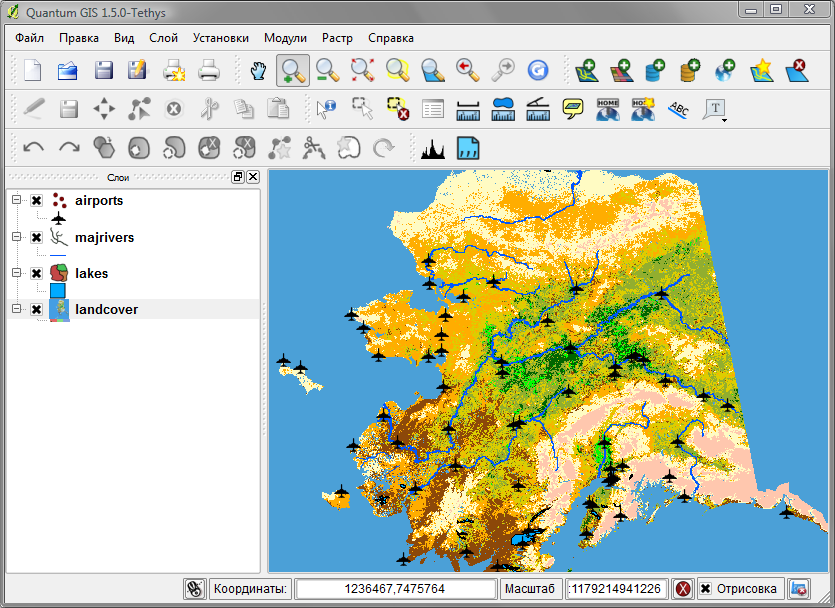
\includegraphics[clip=true, width=12cm]{mapserver_export_qgis}
% \end{center}
% \end{figure}
\begin{figure}[ht]
\centering
  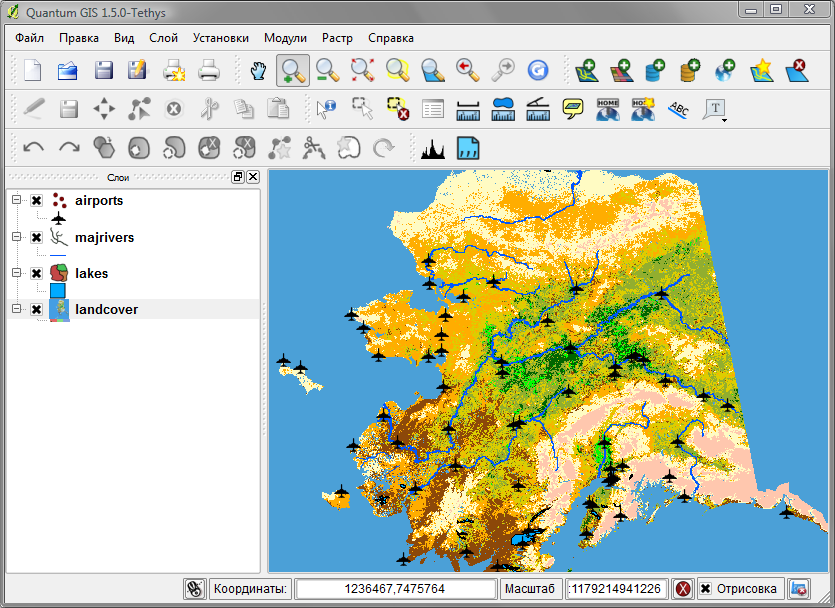
\includegraphics[clip=true, width=12cm]{mapserver_export_qgis}
   \caption{Arrangement des couches d'un fichier de projet QGIS \nixcaption}
  \label{fig:mapserver_export_qgs}
\end{figure}
% In this example, we demonstrate the four steps required to create a simple 
% project file which can be used to create the MapServer map file. 
% We use raster and vector files from the QGIS sample dataset \ref{label_sampledata}.
Dans cet exemple sont présentées les quatre étapes requises pour créer un fichier de projet qui pourra être utilisé pour créer un fichier de carte (mapfile) pour MapServer.Les fichiers vecteurs et rasters proviennent de l'échantillon de jeu de données de Quantum GIS \ref{label_sampledata}.

% \begin{enumerate}
% \item Add the raster layer \filename{landcover.tif} clicking on the 
% \toolbtntwo{mActionAddRasterLayer}{Add Raster Layer} icon.
% \item Add the vector Shapefiles \filename{lakes.shp, majrivers.shp} and 
% \filename{airports.shp} from the QGIS sample dataset clicking on the 
% \toolbtntwo{mActionAddNonDbLayer}{Add Vector Layer} icon.
% \item Change the colors and symbolize the data as you like (For example see 
% Figure~\ref{fig:mapserver_export_qgis})
% \item Save a new project named \filename{mapserverproject.qgs} using 
% \mainmenuopt{File} > \dropmenuopttwo{mActionFileSave}{Save Project}.
% \end{enumerate} 

\begin{enumerate}
\item Ajoutez la couche raster \filename{landcover.tif} en cliquant sur l'icône\\ \toolbtntwo{mActionAddRasterLayer}{Ajouter une Couche Raster}
\item Ajoutez la couche vecteur des shapefiles \filename{lakes.shp, majrivers.shp} et \filename{airports.shp} depuis le jeu de données QGIS en cliquant sur l'icône \toolbtntwo{mActionAddNonDbLayer}{Ajouter une couche Vecteur}.
\item Changer les couleurs et les symboles des données (voir Figure \ref{fig:mapserver_export_qgs})
\item Enregistrez dans un nouveau fichier de projet nommé \filename{mapserverproject.qgs} en utilisant \mainmenuopt{File} > \dropmenuopttwo{mActionFileSave}{Enregistrer le projet}.
\end{enumerate} 

%\subsection{Creating the Map File}
\subsection{Création du fichier .map}

% The tool \filename{msexport} to export a QGIS project file to a MapServer map file is installed in your QGIS binary directory and can be used independently of QGIS. To use it from within QGIS, you need to enable the MapServer Export Plugin first using the Plugin Manager (see Section \ref{sec:load_core_plugin}).

L'outil \filename{msexport} d'exportation se situe dans votre répertoire d'installation de QGIS et peut être utilisé indépendamment de QGIS. Pour l'utiliser à partir du logiciel, vous devez charger l'extension en utilisant le Gestionnaire d'extension. (Voir Section \ref{sec:load_core_plugin}).

% \begin{figure}[ht]
% \begin{center}
  % \caption{Export to MapServer Dialog \nixcaption}
  % \label{fig:mapserver_export_dialog}\smallskip
  % 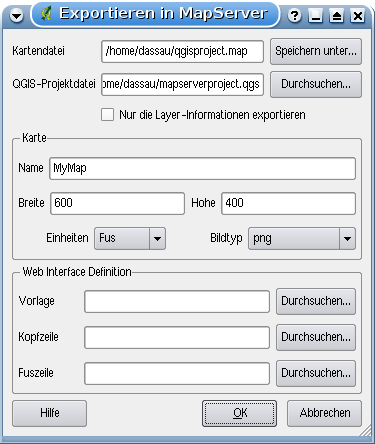
\includegraphics[clip=true, width=9cm]{mapserver_export_dialog}
% \end{center}
% \end{figure}

\begin{figure}[ht]
\centering
  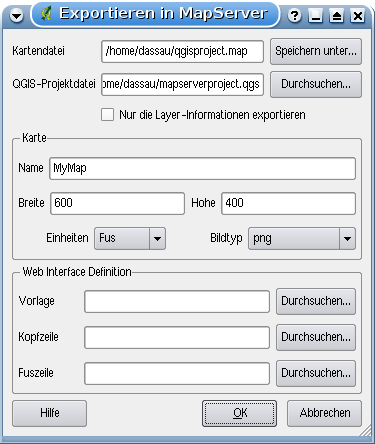
\includegraphics[clip=true, width=8cm]{mapserver_export_dialog}
  \caption{Dialogue d'exportation vers MapServer \nixcaption} \label{fig:mapserver_export_dialog}
\end{figure}

% \begin{description}
% \item [Map file] \mbox{}\\Enter the name for the map file to be created. You can use the button at the right to browse for the directory where you want the map file created. 
% \item [Qgis project file] \mbox{}\\Enter the full path to the QGIS project file (.qgs) you want to export. You can use the button at the right to browse for the QGIS project file.
% \item [Map Name] \mbox{}\\A name for the map. This name is prefixed to all images generated by the mapserver.
% \item [Map Width] \mbox{}\\Width of the output image in pixels.
% \item [Map Height] \mbox{}\\Height of the output image in pixels.
% \item [Map Units] \mbox{}\\Units of measure used for output
% \item [Image type] \mbox{}\\Format for the output image generated by MapServer
% \item [Web Template] \mbox{}\\Full path to the MapServer template file to be used with the map file
% \item [Web Header] \mbox{}\\Full path to the MapServer header file to be used with the map file
% \item [Web Footer] \mbox{}\\Full path to the MapServer footer file to be used with the map file
% \end{description}
\begin{description}
\item [Fichier .map] \mbox{}\\Saisissez le chemin complet du fichier .map que vous voulez exporter. Vous pouvez utiliser le bouton sur la droite pour parcourir votre système.
\item [Fichier projet Qgis] \mbox{}\\Saisissez le chemin complet du fichier projet (.qgs) que vous voulez exporter. Vous pouvez utiliser le bouton sur la droite pour parcourir votre système.
\item [Nom de la carte] \mbox{}\\Un nom pour la carte. Ce nom préfixera toutes les images créées par le serveur.
\item [Largeur de la carte] \mbox{}\\Largeur en pixels de l'image générée.
\item [Hauteur de la carte] \mbox{}\\hauteur en pixels de l'image générée.
\item [Unitées de la carte] \mbox{}\\Unités de mesure utilisées
\item [Type d'image] \mbox{}\\Format de l'image générée par MapServer
\item [Web Template] \mbox{}\\Chemin complet vers le fichier MapServer template à utiliser
\item [Web en-tête] \mbox{}\\Chemin complet vers le fichier d'en-tête de MapServer à utiliser
\item [Web bas de page] \mbox{}\\Chemin complet vers le fichier de bas de page MapServer à utiliser
\end{description}

% Only the \filename{Map file} and \filename{QGIS project file} inputs are required to create a map file, however by omitting the other parameters, 
% you may end up creating a non-functional map file, depending on your intended use. Although QGIS is good at creating a map file from your project file, 
% it may require some tweaking to get the results you want. For this example, we will create a map file using the project file \filename{mapserverproject.qgs} we just created (see Figure~\ref{fig:mapserver_export_dialog}):

Seulement le \filename{fichier .map} et le \filename{fichier de projet QGIS} sont requis pour créer un fichier .map, vous risquez cependant d'obtenir un fichier inutilisable selon ce que vous désirez en faire. Bien que QGIS soit en mesure de créer les fichiers .map, votre projet nécessite peut-être des adaptions pour obtenir le résultat escompté. Créons un fichier .map en utilisant le projet \filename{mapserverproject.qgs} que nous avons créé (voir Figure~\ref{fig:mapserver_export_dialog}):

% \begin{enumerate}
  % \item  Start the MapServer dialog (see Figure \ref{fig:mapserver_export_dialog}) by clicking the \toolbtntwo{mapserver_export}{MapServer Export} icon in the toolbar menu.
  % \item Enter the name (e.g., \filename{qgisproject.map}) for your new map file.
  % \item Browse and find the QGIS project file (e.g., \filename{mapserverproject.qgs}) you previously saved.
  % \item Enter a name (e.g., \filename{MyMap}) for the map.
  % \item Enter the width and height (e.g., \filename{600} for the width and \filename{400} for the height) for your output image.
  % \item For this example, the layers are in meters, so we change the units to meters.
  % \item Choose ``png'' for the image type.
  % \item Click \button{OK} to generate the new map file \filename{qgisproject.map}. 
  % QGIS displays the success of your efforts.
% \end{enumerate}

\begin{enumerate}
  \item Ouvrez l'extension en cliquant sur l'icône \toolbtntwo{mapserver_export}{Exporter vers }.
  \item Entrez le nom \filename{qgisproject.map} pour votre nouveau fichier .map.
  \item Sélectionnez le projet QGIS \filename{mapserverproject.qgs} que vous venez d'enregistrer.
  \item Entrez un nom \filename{MaCarte} pour la carte.
  \item Entrez \filename{600} pour la largeur et \filename{400} pour la hauteur.
  \item Nos couches sont en mètres, l'unité de mesure sera donc le mètre.
  \item Choisissez ``png'' pour le type d'image.
  \item Cliquez sur \button{OK} pour générer le nouveau fichier \filename{qgisproject.map}. 
  QGIS affiche le résultat de vos efforts.
\end{enumerate}

% You can view the map file in any text editor or visualizer. If you take a look, you'll notice that the export tool adds the metadata needed to enable our map file for WMS. 
Vous pouvez visualiser le fichier .map dans un éditeur de texte. Si vous le faites, vous remarquerez que l'outil d'exportation ajoute les métadonnées nécessaires à l'utilisation du protocole WMS.

%\subsection{Testing the Map File}
\subsection{Test du fichier .map}

% We can now test our work using the \filename{shp2img} tool to create an image from the map file. The \filename{shp2img} utility is part of MapServer and FWTools.
% To create an image from our map:

Nous pouvons maintenant tester notre travail en utilisant l'outil \filename{shp2img} pour créer une image tirée du fichier .map. Cet outil est présent dans MapServer et FWTools. 
Pour créer une image :

% \begin{itemize}
% \item Open a terminal window
% \item If you didn't save your map file in your home directory, change to the folder where you saved it.
% \item Run \filename{shp2img -m qgisproject.map -o mapserver\_test.png} and display the image 
% \end{itemize}

\begin{itemize}
\item Ouvrez une console de commande
\item Si vous n'avez pas sauvegardé votre fichier dans votre répertoire personnel, déplacez vous vers le bon dossier
\item Lancez \filename{shp2img -m qgisproject.map -o mapserver\_test.png} et affichez l'image
\end{itemize}
 
% This creates a PNG with all the layers included in the QGIS project file.In addition, the extent of the PNG will be the same as when we saved the 
% project. As you can see in Figure~\ref{fig:mapserver_export_test}, all information except the airport symbols are included.
Une image PNG est créée avec toutes les couches du projet QGIS. De plus, l'étendue du PNG sera la même que celle du projet. Comme vous le voyez sur la figure~\ref{fig:mapserver_export_test}, toutes les informations, à l'exception des symboles des aéroports, sont incluses.

% \begin{figure}[ht]
% \begin{center}
  % \caption{Test PNG created by shp2img with all MapServer Export layers \nixcaption}
  % \label{fig:mapserver_export_test}\smallskip
  % 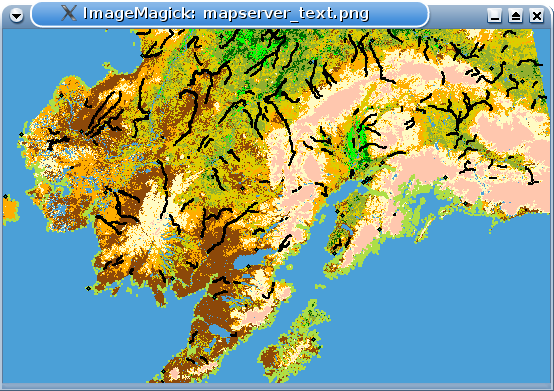
\includegraphics[clip=true, width=12cm]{mapserver_export_test}
% \end{center}
% \end{figure}
\begin{figure}[ht]
\centering
  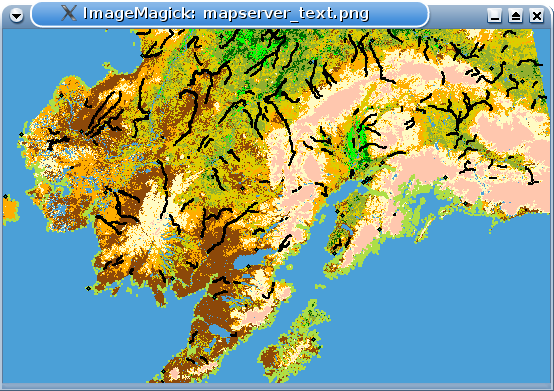
\includegraphics[clip=true, width=10cm]{mapserver_export_test}
  \caption{Image PNG créée par shp2img avec toutes les couches\nixcaption}
  \label{fig:mapserver_export_test}
\end{figure}

% If you plan to use the map file to serve WMS requests, you probably don't have to tweak anything. If you plan to use it with a mapping template or a
% custom interface, you may have a bit of manual work to do. To see how easy it is to go from QGIS to serving maps on the web, take a look at
% Christopher Schmidt's 5 minute flash video. He used an older version of QGIS (version 0.8), but the demo applies equally well to newer versions.
% \footnote{\url{http://openlayers.org/presentations/mappingyourdata/}}
Si vous comptez utiliser ce fichier .map pour fournir un service WMS, vous n'aurez probablement rien d'autre à modifier. Par contre si vous comptez l'utiliser comme modèle ou dans une interface personnalisée vous aurez un peu plus de travaux manuels à effectuer. Vous pouvez jeter un oeil sur cette vidéo de Christopher Schmidt (version 0.8 de QGIS mais cela reste valable).
\footnote{\url{http://openlayers.org/presentations/mappingyourdata/}}
